\documentclass[a4paper, 11pt, ngerman, fleqn]{article}
\usepackage[utf8]{inputenc}
\usepackage{babel}
\usepackage{ngerman}
\usepackage{coordsys,logsys,color}
\usepackage{german,fancyhdr}
\usepackage{hyperref}
\usepackage{texdraw}				
\usepackage[T1]{fontenc}					
\usepackage{amsmath,amsfonts,amssymb}	
\usepackage[normalem]{ulem}	
\usepackage{listings}
\usepackage{graphicx}

\definecolor{darkblue}{rgb}{0,0,.6}
\definecolor{glossb}{rgb}{0,0,0.38}
\hypersetup{colorlinks=true, breaklinks=true, linkcolor=darkblue, menucolor=darkblue, urlcolor=darkblue, citecolor=darkblue}

\lhead{\sc{Reviewdokument PECTO}}

\pagestyle{fancy}

\renewcommand{\familydefault}{cmss}

\definecolor{fgcgray}{rgb}{0.4, 0.4, 0.4}
\definecolor{darkblue}{rgb}{0,0,.6}
\definecolor{glossb}{rgb}{0,0,0.38}
\newcommand{\titlefont}[1]{\textcolor{black}{\fontseries{bx}\fontshape{n}\fontsize{30}{0pt} \selectfont #1}}
\newcommand{\titlepagef}[1]{\textcolor{black}{\fontseries{bx}\fontshape{n}\fontsize{14}{0pt} \selectfont #1}}

\newcommand{\gloss}[1]{\textcolor{glossb}{\fontsize{11}{0pt}\selectfont #1}}



\addtolength{\oddsidemargin}{-1.0cm}
\addtolength{\evensidemargin}{-1.0cm}
\addtolength{\headwidth}{2.0cm}
\addtolength{\textwidth}{2.0cm}

\setlength{\parindent}{0cm}

\renewcommand{\labelitemi}{$\circ$}
\renewcommand{\labelitemii}{$\diamond$}

\newcommand{\spaceline}[1][8pt]{\vskip #1}
\newcommand{\attrname}[1]{\textcolor{fgcgray}{\scriptsize #1}}

\newcommand{\comment}[1]{\spaceline[5pt] \textcolor{fgcgray}{\scriptsize #1} \spaceline[15pt]}

\makeatletter

\newcommand*{\project}[1]{\gdef\@project{#1}}

\usepackage[]{siunitx}


\def\@maketitle{
  %\begin{titlepage}
   
  \begin{center}
      \titlepagef{Softwareprojekt 2016}
      \spaceline
  \end{center}
  
  \begin{center}
      \parbox{\textwidth}{
        \spaceline
        \centering{\titlefont{\@title}}
        \par
        \spaceline
      }
  \end{center}
  
  \begin{center}
    \titlepagef{Rapid Layer-2 Encryption Framework}
    \spaceline[2em]
  \end{center}
  
  \begin{center}
  \begin{tabbing}
  Yannic Faulwetter \qquad \=
  Michael Fuchs \qquad \=
  Milan Haverkock \qquad \=
  Felix Seidel \\
  Daniel Scheliga
  \>Tobias Schubert
  \>Jörn Weisensee  
  \>Nils Winkelbach
  \end{tabbing}
  \end{center}
 
  
  \spaceline[3em] {
    \begin{flushright}
    \begin{tabular}[t]{rl}
      \attrname{letzte Änderung:} & \@date
    \end{tabular}
    \end{flushright}
    \par
  }
  \spaceline[5.5em]
  %\end{titlepage}
}

\begin{document}
\title{Reviewdokument: PECTO}
\vspace{3 in}
\maketitle
\clearpage
\tableofcontents
\clearpage


\section*{Reviewdokument der Implementierungsphase}
In diesem Reviewdokument sollen die Ergebnisse des Softwareprojektes in der zweiten Phase betrachtet werden.
Insbesondere wird auf wichtige Designentscheidungen eingegangen, die bei der Erarbeitung des Feinentwurfs getroffen wurde.
Als Anhang liegt die komplette, von Doxygen generierte, Entwicklerdokumentation bei.

Neben den Erfolgen bei der Entwicklung sind zudem die Probleme dokumentiert, die während der zweiten Iteration zustande kamen. Einige davon blieben auch als Aufgabe für den nächsten Sprint bestehen. 

Als Vorbereitung für die nächste Iteration werden die finalen Aufgaben festgelegt, welche noch bis zur Beendigung des Projektes umgesetzt werden müssen. 

\clearpage
\section{Ziele und Relevanz des Frameworks PECTO}
PECTO (Paket EnCryption on layer TwO) ist ein Framework, dass es ermöglicht, verschiedene zu schützende, \gloss{rote Netze} sicher zu verbinden.  
Da hier verschiedenartig sturkturierte Netzwerke mit unterschiedlichen Kommunikationsprotokollen arbeiten, agiert es als ein Gateway, welches die Kommunikation zwischen roten Netzen über ein unsicheres, \gloss{schwarzes Netz} ermöglicht. 
Dabei werden die Pakete, welche zwischen roten Netzen versandt werden, verschlüsselt über ein \gloss{schwarzes Netz} übertragen.
Im Gegensatz zu schon verbreiteten \gloss{VPN}-Lösungen erfolgt die Verschlüsselung jedoch auf Layer-2 des ISO/OSI-Schichtenmodells, behandelt also Ethernet-Frames statt IP-Pakete.

PECTO kann zur Absicherung von lokalen Netzwerken verwendet werden, ohne Spezialhardware nutzen zu müssen.

\clearpage
\section{Ziele im beim Entwurf PECTOs}
An das zu entwickelnde Framework PECTO stellten wir verschiede Anforderungen, insbesondere auch an die Performance und Sicherheit. 
Diese finden sich auch verschiedenen Stellen in den Entwurfsentscheidungen wieder.  
Dabei konkurriert der Sicherheitsgedanke, welcher nach möglichst einfachem Code strebt, stets mit dem Wunsch nach hoher Performance.
Um einen guten Ausgleich zu finden, werden alle Komponenten zunächst auf gute Verständlichkeit des Codes optimiert.
Sollten sich beim Profiling Probleme zeigen, werden diese Stellen gezielt überarbeitet.

\subsection*{Verwendete Muster}
Zur Realisierung von PECTO werden folgende Entwurfsmuster verwendet:

\begin{description}
	\item[Inversion of Control (IoC)] 
	Um das Schichtenmodell umsetzen zu können und zyklische Abhängigkeiten zu vermeiden, wird Inversion of Control eingesetzt. 
	Die tiefere Schicht stellt dafür jeweils Interfaces bereit, die von den höheren Schichten implementiert werden. 
	Der sich dadurch ergebende Overhead ist in der Regel zu vernachlässigen.
	Insbesondere überwiegen die Vorteile durch eine bessere Entkoppelung.
	Wenn sich Performance-Probleme ergeben, kann davon abgewichen werden.
	
	\item[Strategy Pattern]
	An verschiedenen Stellen im Entwurf können verschiedene Algorithmen verwendet werden. 
	Damit dies konfgurierbar ist, wird das Strategy Pattern verwendet.
	Ein Beispiel hierfür ist die Wahl des Verschlüsselungsalgorithmus, der zu Debuggingzwecken und für Erweiterbarkeit verschiedenartig gewählt werden kann.
	Zur Auswahl stehen zum Beispiel AES-GCM, eine unsichere XOR-Verschlüsselung oder gar keine Verschlüsselung. 
	
	\item[Exceptions]
	Zur Vereinfachung des Codes werden Exceptions eingesetzt.
	Diese sind immer dann auszugeben, wenn ein unerwartetes Ereignis eingetreten ist.
	Da der Einsatz von Exceptions einen erheblichen Overhead zur Folge haben kann, wenn zu viele von ihnen geworfen werden, müssen für besonders performance-kritische Funktionen immer zwei Schnittstellen zur Verfügung stehen.
	Die erste dieser Schnittstellen löst die Exceptions aus, während die zweite über Rückgabewerte entscheidet ob die Funktion erfolgreich ausgeführt wurde.
	
	\item[Code Contracts]
	Jede Methode, die zu einer öffentlichen Schnittstelle gehört, validiert ihre Parameter und Ausgaben.
	Unerwartete Eingaben, beispielsweise Nullzeiger, müssen erkannt werden und zu einer Exception führen.
	Ebenfalls sollen alle Ausgaben einer einfachen Plausibilitätsprüfung unterzogen werden. 
	Auch hier liegt besonderes Augenmerk auf Nullzeigern.
	So wird sichergestellt, dass keine unerwarteten Rückgabewerte zu Fehlern an anderer Stelle führen können.
	Ausnahmen bilden einige performancekritische Funktionen, die in auch eine Variante bereitstellen, die keine Prüfung durchführt.
\end{description}

\clearpage
\section{Bugreview}
Im Laufe des letzten Sprintes sind wir auf verschiedene Probleme gestoßen.
Die meisten davon konnten leicht wieder behoben werden, allerdings bleibt insbesondere ein schwerwiegendes Problem bestehen.

\subsection{Receive Side Scaling (RSS) im schwarzen Netz}
In diesem Abschnitt wird das größte Problem, dass es noch zu lösen gilt, beschrieben.
Dabei handelt es sich um die verwendete Technologie, um Pakete zwischen verschiedenen Warteschlangen zu verteilen.

\begin{description}
	
	\item[Receive Side Scaling] 
	Receive Side Scaling ist eine Technologie, bei der die Netzwerkkarte empfangene Pakete auf verschiedene Warteschlangen verteilt.
	Diese wird von PECTO benutzt, um das Load Balancing zwischen verschiedenen Threads umzusetzen.
	
	\item[Problembeschreibung]
	RSS nutzt verschiedene Informationen aus höheren Schichten, z.B. IP-Adressen, um die Pakete sinnvoll an verschiedende Warteschlangen zu verteilen. 
	Wenn jedoch ein PECTO-Paket aus dem schwarzen Netz empfangen wird, kann auf diese Informationen zwangsläufig noch nicht zugegriffen werden.
	Damit kann auch kein Balancing stattfinden.
	
	\item[Workaround]
	Einige teurere Netzwerkkarten können RSS auch anhand des gesamten Paketes ausführen, jedoch ist dies keine Lösungsmöglichkeit, welche für die Realisierung dieses Systems in Frage kommt.
	Ein anderer Workaround ist das Setzen von benutzerdefinierten Filtern, sogenannten Flex Filters, auf dem Netzwerkinterface, die verschiedene Pakete explizit den verschiedenen Queues zuordnen. 
\end{description}

\subsection{Fehlende Features}
Bis zur Finialisierung PECTOs müssen noch einige Features implementiert werden.
Diese sind im Folgenden aufgelistet.

\subsubsection{Fehler in bestehenden Programmteilen}
Durch verschiedene Test haben sich in verschiedenen Programmteilen Fehler herausgestellt. 
Diese im folgenden aufgeführten Probleme konnten noch nicht behoben werden.

\begin{description}

\item[Receive Side Scaling:] Durch die Verschlüsselung der Pakete wurden alle Informationen, auf die das RSS zugreifen würde um Aufteilungsentscheidungen zu treffen unkenntlich gemacht. Somit ist das RSS nicht in der Lage eine geeignete bzw. sinnvolle Verteilung der Paket auf die Warteschlangen zu gewährleisten.

\item[XOR-Verschlüsselung:] Diese Art der Verschlüsselung wurde implementiert um das Debuggen zu erleichtern und auftretende Fehler in der Crypto-Komponente genauer lokalisieren zu können. Das Problem hierbei ist, dass die Verschlüsselung zu langsam für die angestrebte Performance des Framewoks ist.

\end{description}

\subsubsection{Fehlende MUSS-Funktionen}
Auf Grund anderer elementarer Anforderungen an das System, mussten folgende Funktionen in die dritte Iteration verschoben werden.

\begin{description}

% Verbindungsaufbau
\item[Authentisierung:] Zwei Instanzen einer Gruppe müssen einander identifizieren, indem sie sicherstellen, dass die jeweils andere Instanz dasselbe Kennwort zum Schutz der roten Netzgruppe kennt.

\item[Schlüsselaustausch für Unicast:] Zwei Instanzen einer Gruppe handeln einen Schlüssel aus, der zum Chiffrieren und Dechiffrieren der Pakete genutzt wird, welche zwischen den beiden Instanzen ausgetauscht werden. 
Dabei müssen folgende Sicherheitsanforderungen erfüllt sein: Authentizität, Vertraulichkeit, Perfect Forward Secrecy.

\item[Schlüsselaustausch für Broad- und Multicast:] Alle Instanzen erhalten einen Gruppenschlüssel, welcher zuvor erstellt und verteilt wurde. 
Dieser Gruppenschlüssel wird zum Chiffrieren und Dechiffrieren derjenigen Pakete genutzt, die an alle Instanzen der Gruppe weitergeleitet werden.
Dabei müssen folgende Sicherheitsanforderungen erfüllt sein:
Authentizität, Vertraulichkeit, Perfect Forward Secrecy.

\item[Logging:] Fehler beim Schlüsselaustausch müssen protokolliert werden, da diese auf
einen Angriff auf das System hindeuten können.

%Zugriffskontrolle
\item[Kontrollierter Zugriff:] Das System isoliert die geschützte Netzgruppe vollständig, d.h.
es dürfen keine Pakete zwischen Geräten im schwarzen und roten Netz ausgetauscht
werden.
\end{description}  

\subsubsection{Fehlende KANN-Funktionen}
Die Kann-Funktionen wurden in die dritte Iteration aufgenommen, da die Abarbeitung der Musskriterien noch nicht voll abgeschlossen ist. 

\begin{description}

\item[Automatischer Netzaufbau:] Eine Instanz des Systems kann in dem schwarzen Netz
automatisch nach anderen Instanzen suchen, welche die gleiche Netzgruppenkennung
haben.

\item[Rekeying:] Der Schlüssel zur Sicherung der Verbindungen zwischen einzelnen Instanzen kann regelmäßig erneuert werden.

\item[Statistiken:] Die Instanzen können Statistiken über die Auslastung, Paketeigenschaften und Fehlern führen.
\end{description}

\clearpage
\section{Umgesetzter Entwurf}

Da zum bisherigen Zeitpunkt einige Teile des Systems noch nicht implementiert sind, ist auch der Entwurf noch einfacher gehalten.
Es beschränkt sich dabei jedoch nur auf die Teile, die zum Framework gehören, also isoliert von der konkreten Verschlüsselungsanwendung auch eingesetzt werden können.
Im Vergleich zum Grobentwurf fehlt noch das Dispatch- und CPH-Modul. 
Abhängigkeiten der Tools, die zum Testen verwendet werden, sowie die des Hauptprogramms, sind darin nicht aufgezeigt.

Die existenten Module sollen im Folgenden einzeln beschrieben werden.

\subsection{Network Abstraction}
In der Netzwerkabstraktionsschicht existieren folgende Klassen (siehe Abbildung 1):

\begin{figure}
	\begin{center}
		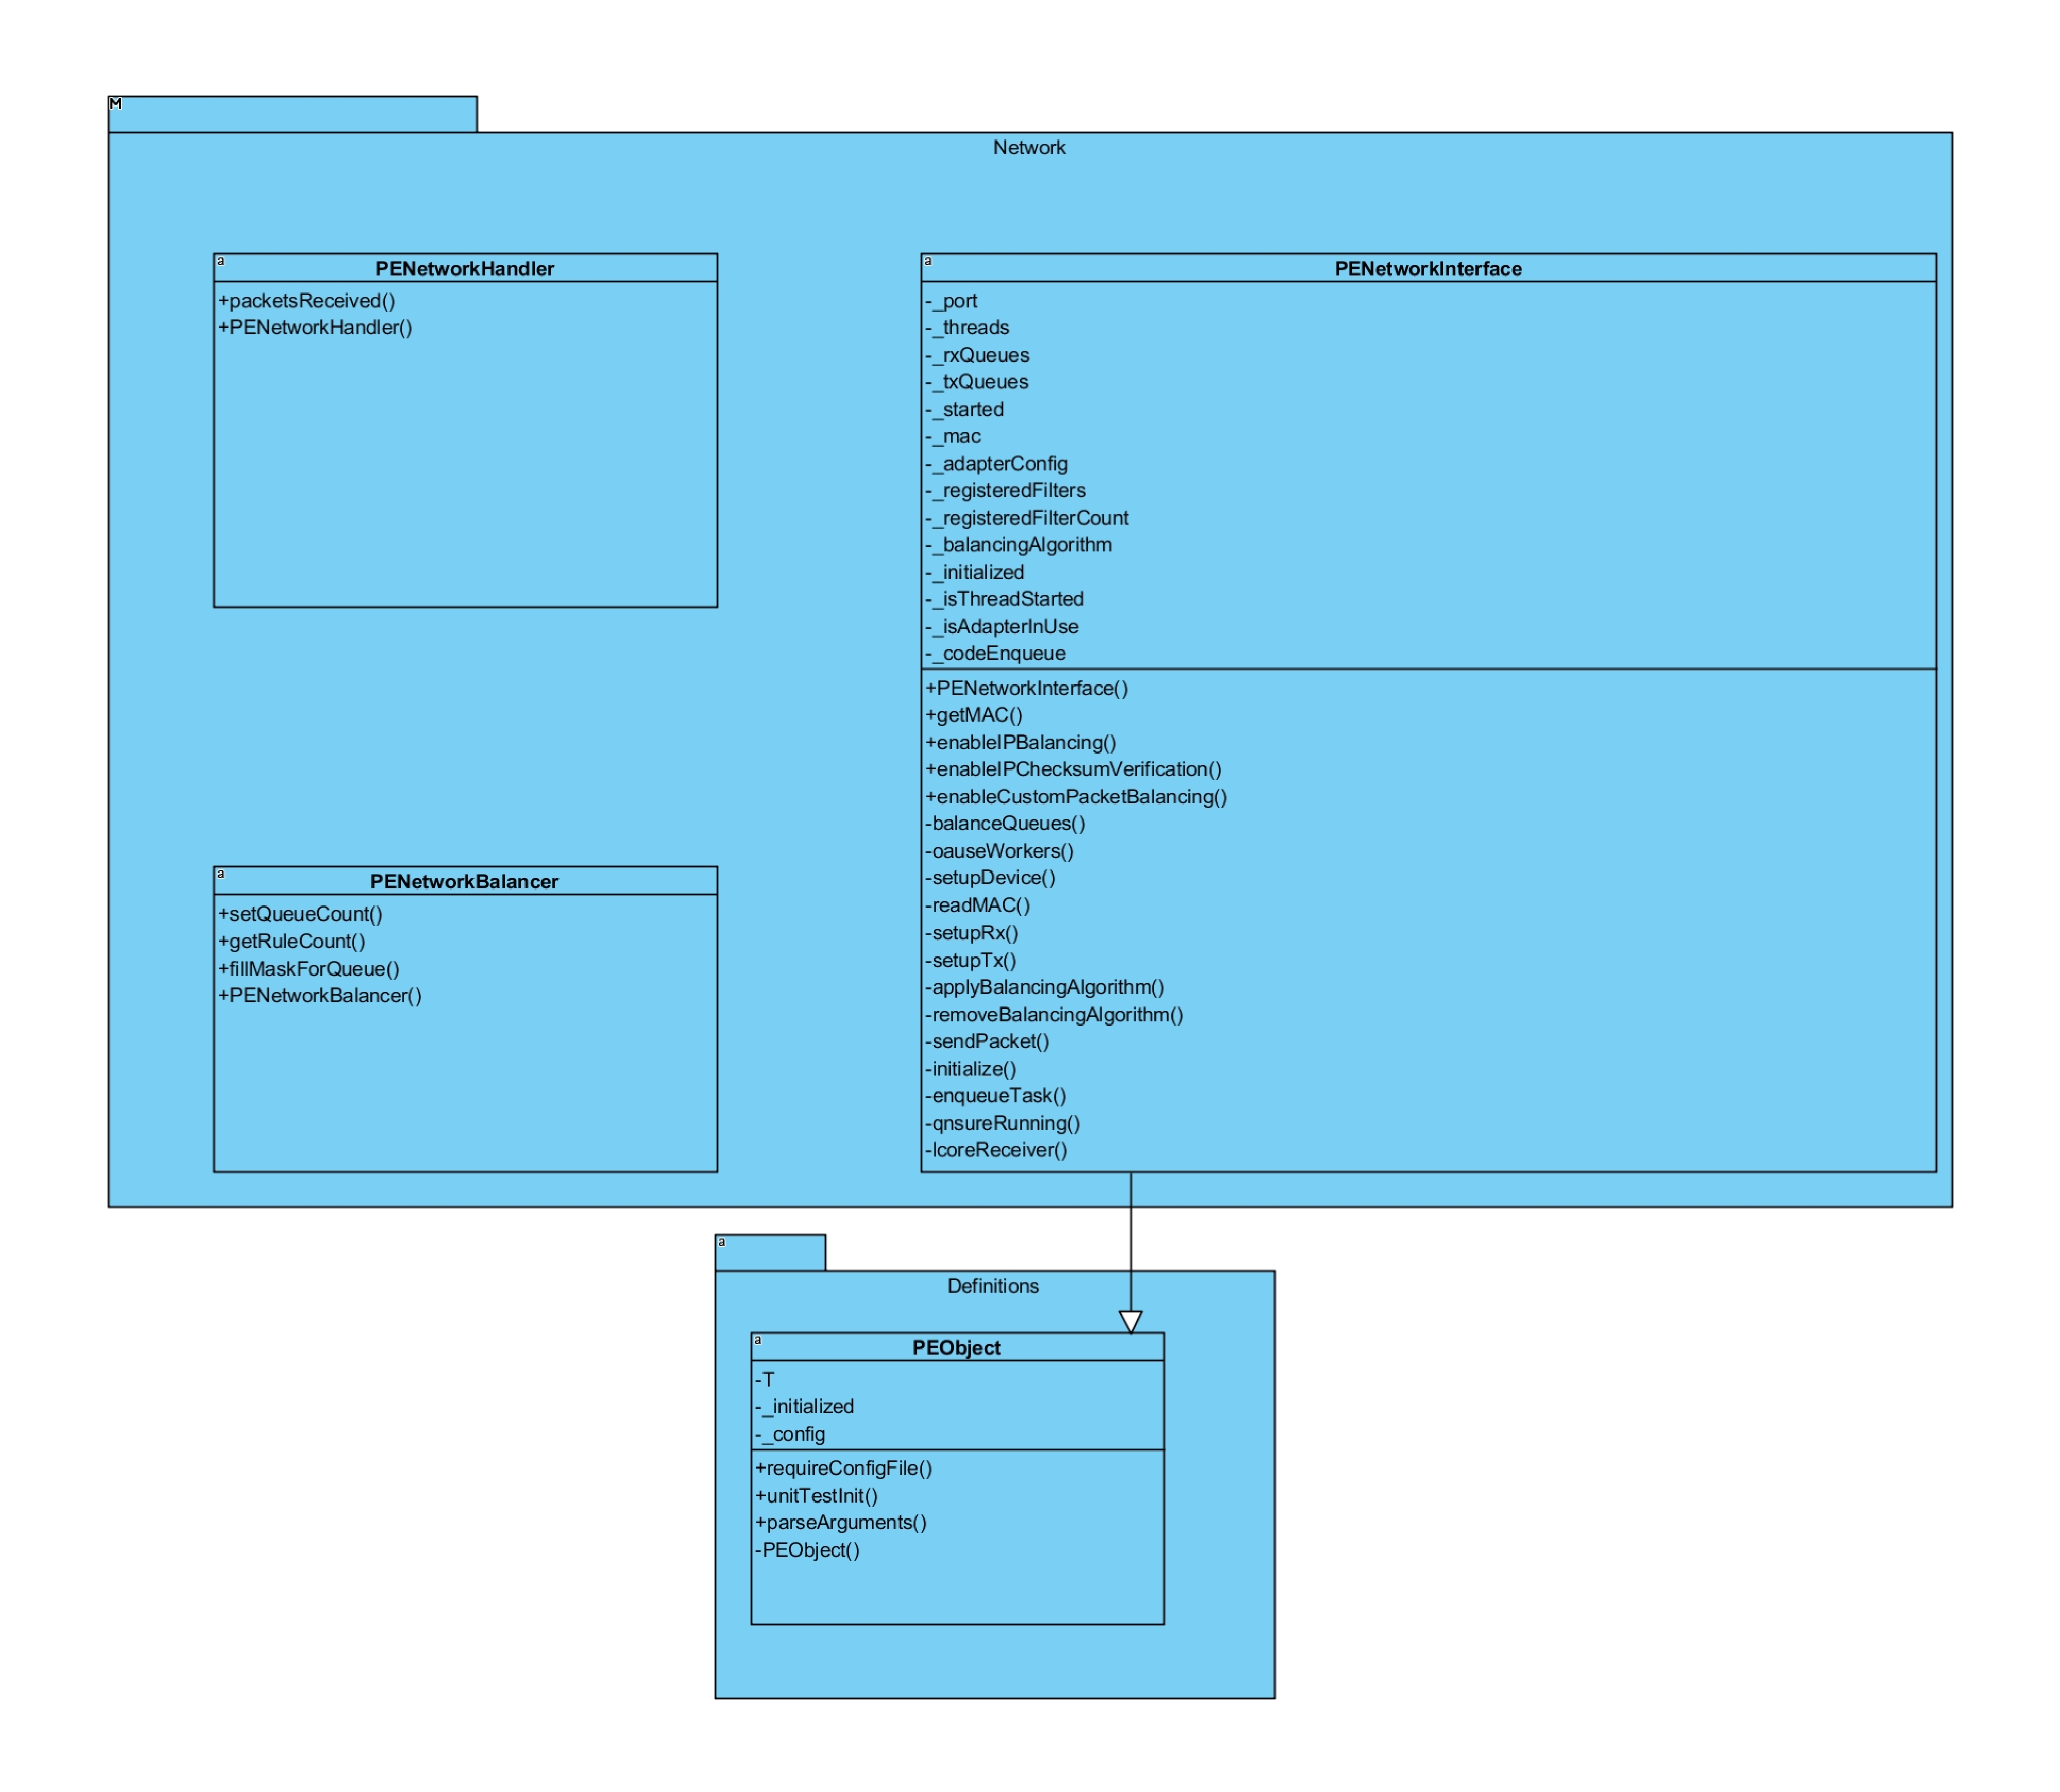
\includegraphics[width=1 \textwidth]{figures/Network.pdf}
		\caption{Network Abstraction}
	\end{center}
\end{figure}

\begin{description}
	\item[PENetworkInterface] 
	\texttt{PENetworkInterface} bildet die Hauptklasse in diesem Modul. 
	Jede Instanz der Klasse verwaltet einen Netzwerkport.
	Zudem erlaubt sie, mehrere Netzwerkinterfaces vom selben Thread aus abzufragen, sowie ein Netzwerkinterface von beliebig vielen Threads abfragen zu lassen.
	Empfangene Pakete werden an eine Implementierung des Interfaces \texttt{PENetworkHandler} weitergereicht.
	
	\item[PENetworkHandler]
	Ein \texttt{PENetworkHandler} verarbeitet eingehende Pakete. 
	Dieses Interface wird innerhalb PECTOs von verschiedenen Klassen in der Forwarding-Komponente implementiert.
	
	\item[PENetworkBalancer]
	Um die Verteilung von Paketen auf verschiedene Verarbeitungsthreads zu ermöglichen, wird ein \texttt{PENetworkBalancer} genutzt.
	Dieser kann abhängig von der Anzahl der zur Verfügung stehenden Empfangsschlangen die Pakete verteilen, indem er ein Muster vorgibt, dem ein Paket entsprechen muss.
	Für die verschiedenen Schlangen werden unterschiedliche Muster angegeben, sodass die Pakete auf verschiedene Threads aufgeteilt, und von diesen bearbeitet werden können. 
\end{description}


\subsection{Memory}
In der Speicherabstraktionsschicht existieren folgende Kassen (siehe Abbildung 2):

\begin{figure}
	\begin{center}
		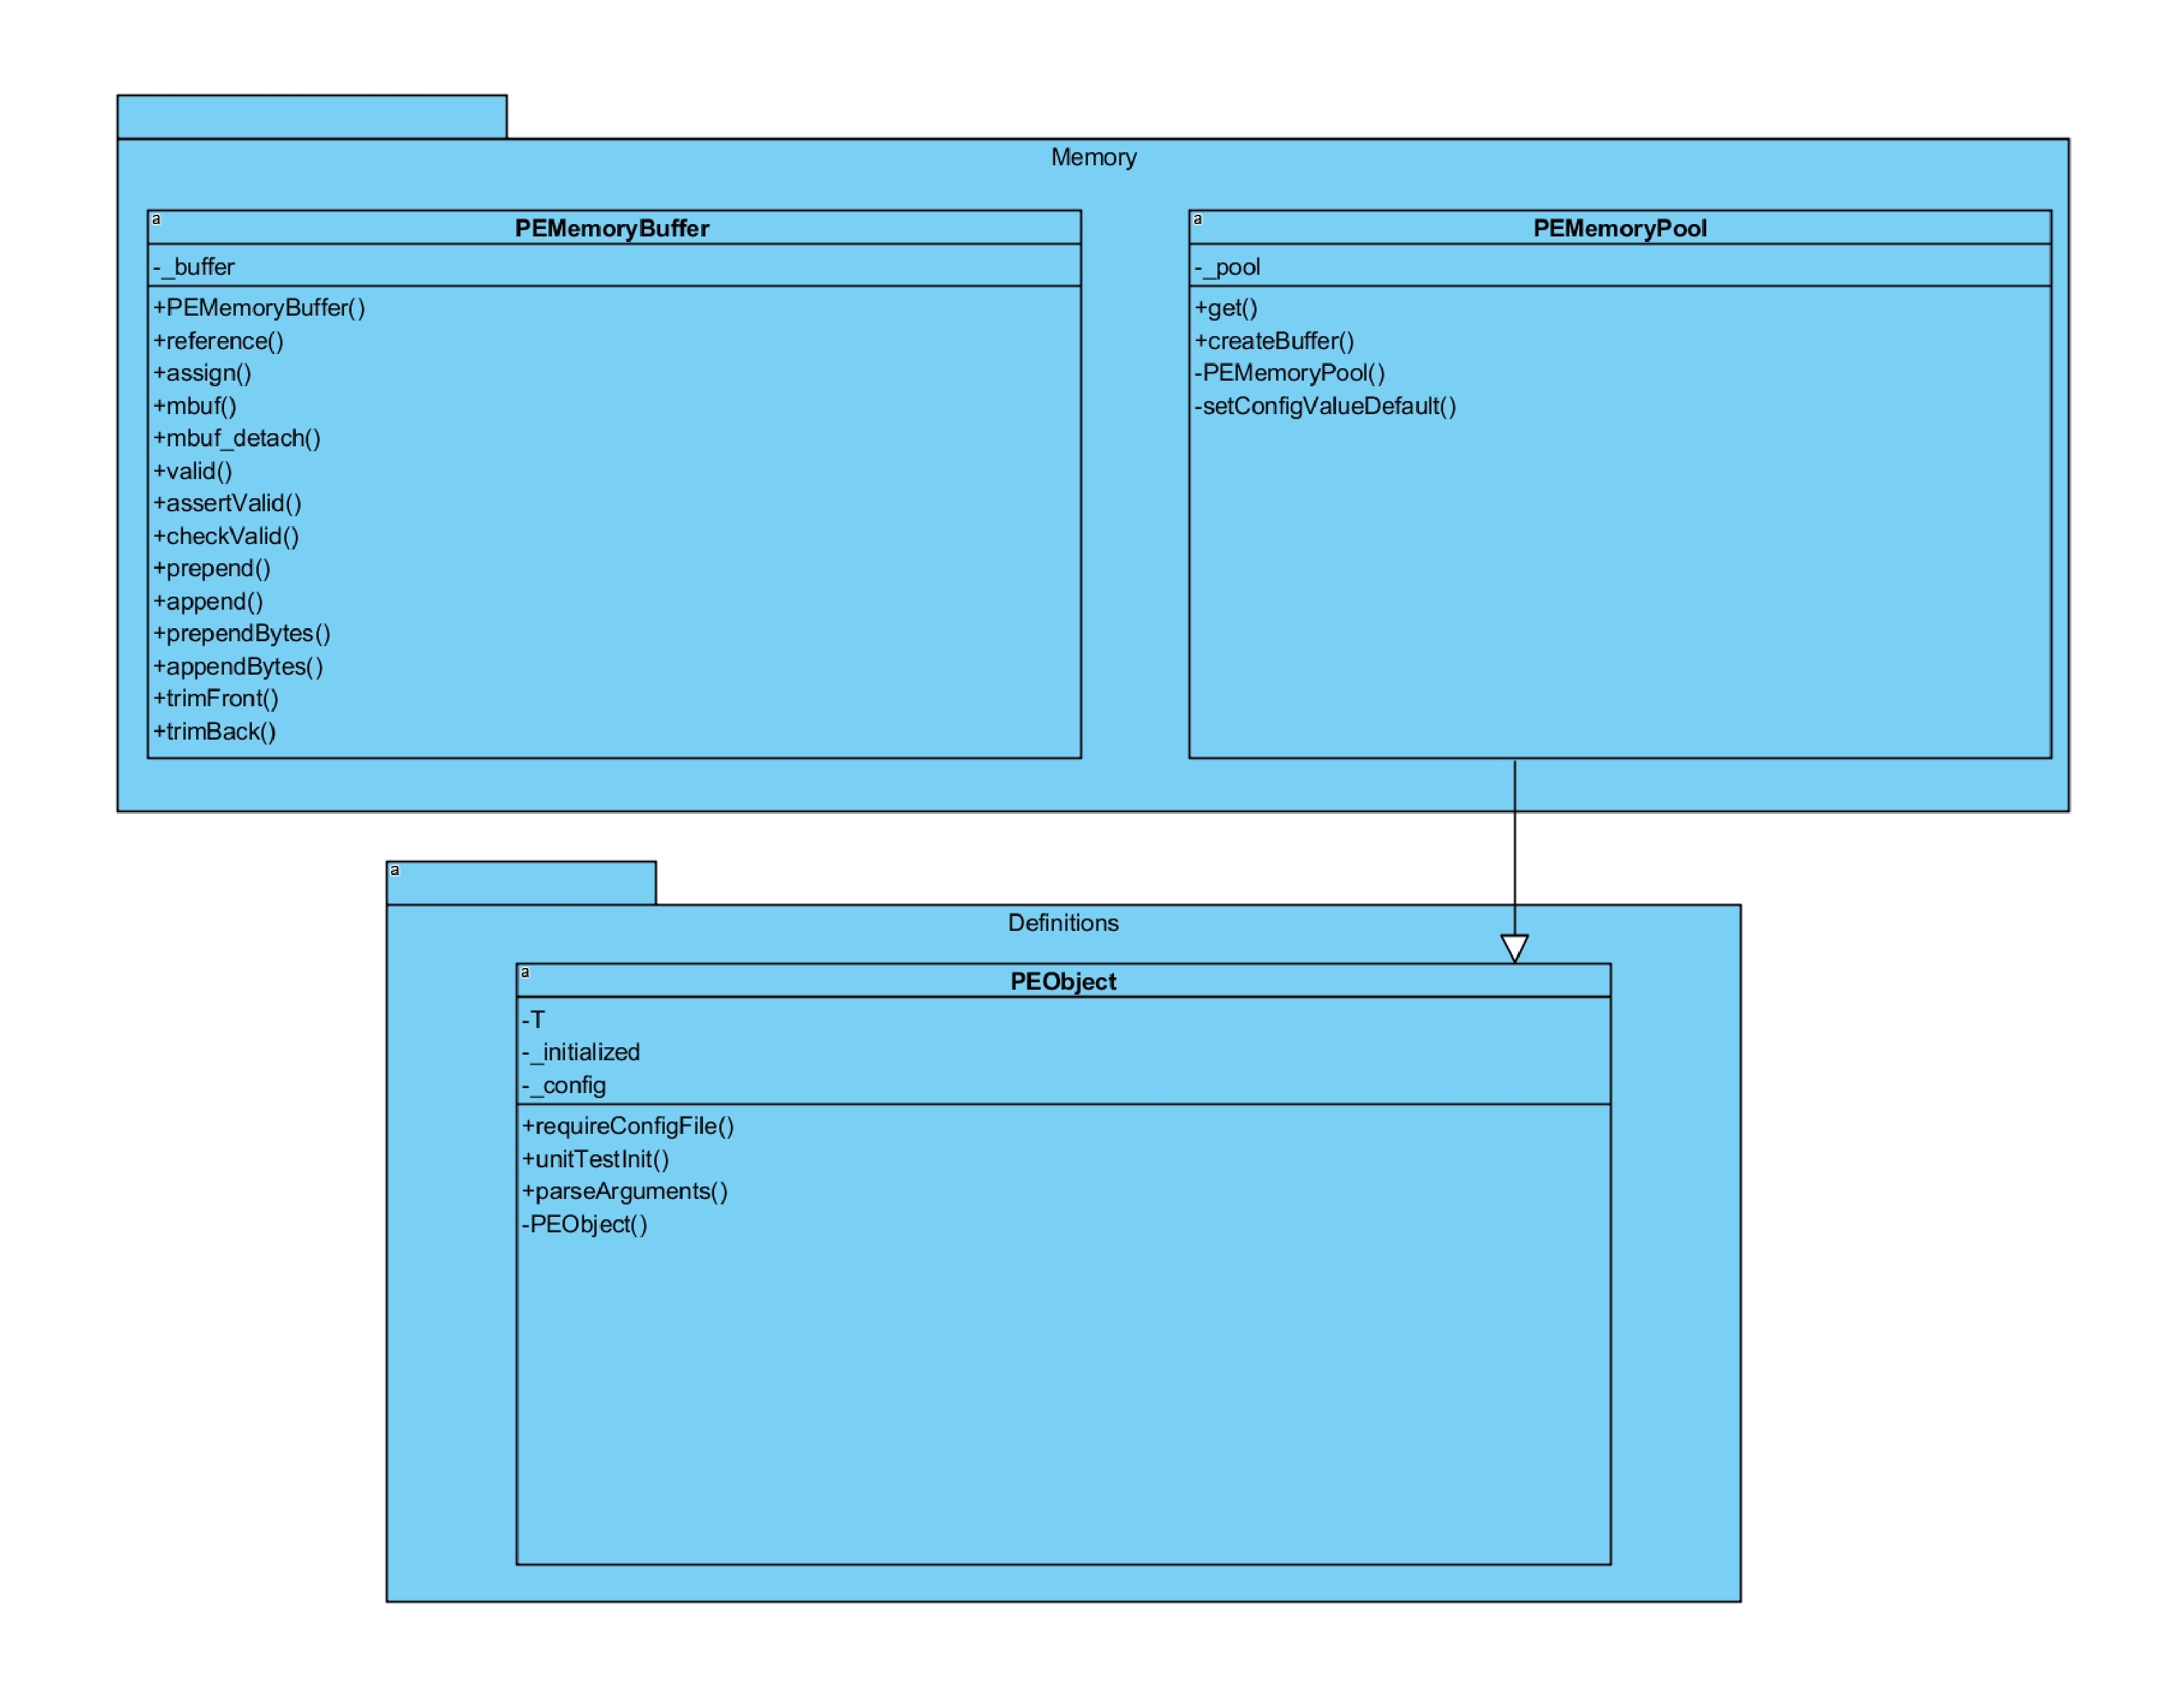
\includegraphics[width=1 \textwidth]{figures/Memory.pdf}
		\caption{Memory}
	\end{center}
\end{figure}

\begin{description}
	\item[PEMemoryPool] 
	\texttt{PEMemoryPool} ist ein Singleton, dass einen Pool von \texttt{PEMemoryBuffer} bereitstellt.
	Dieser Pool ermöglicht die sehr schnelle Allokation von \texttt{PEMemoryBuffer}, sodass mit hoher Geschwindigkeit neue Pakete erzeugt werden können.
	Zudem benutzen die DPDK-Funktionen den Pool, um Paketspeicher nach dem Senden wieder freizugeben.
	
	
	\item[PEMemoryBuffer]
	Ein \texttt{PEMemoryBuffer} stellt meistens ein Paket dar, kann aber auch beliebige Daten aufnehmen.
	Es können Daten angehangen oder vorangestellt werden, was insbesondere beim Umgang mit Paketen sehr nützlich ist.
\end{description}

\subsection{Forwarding}
In der Forwarding-Komponente existieren folgende Klassen (siehe Abbildung 3):

\begin{figure}
	\begin{center}
		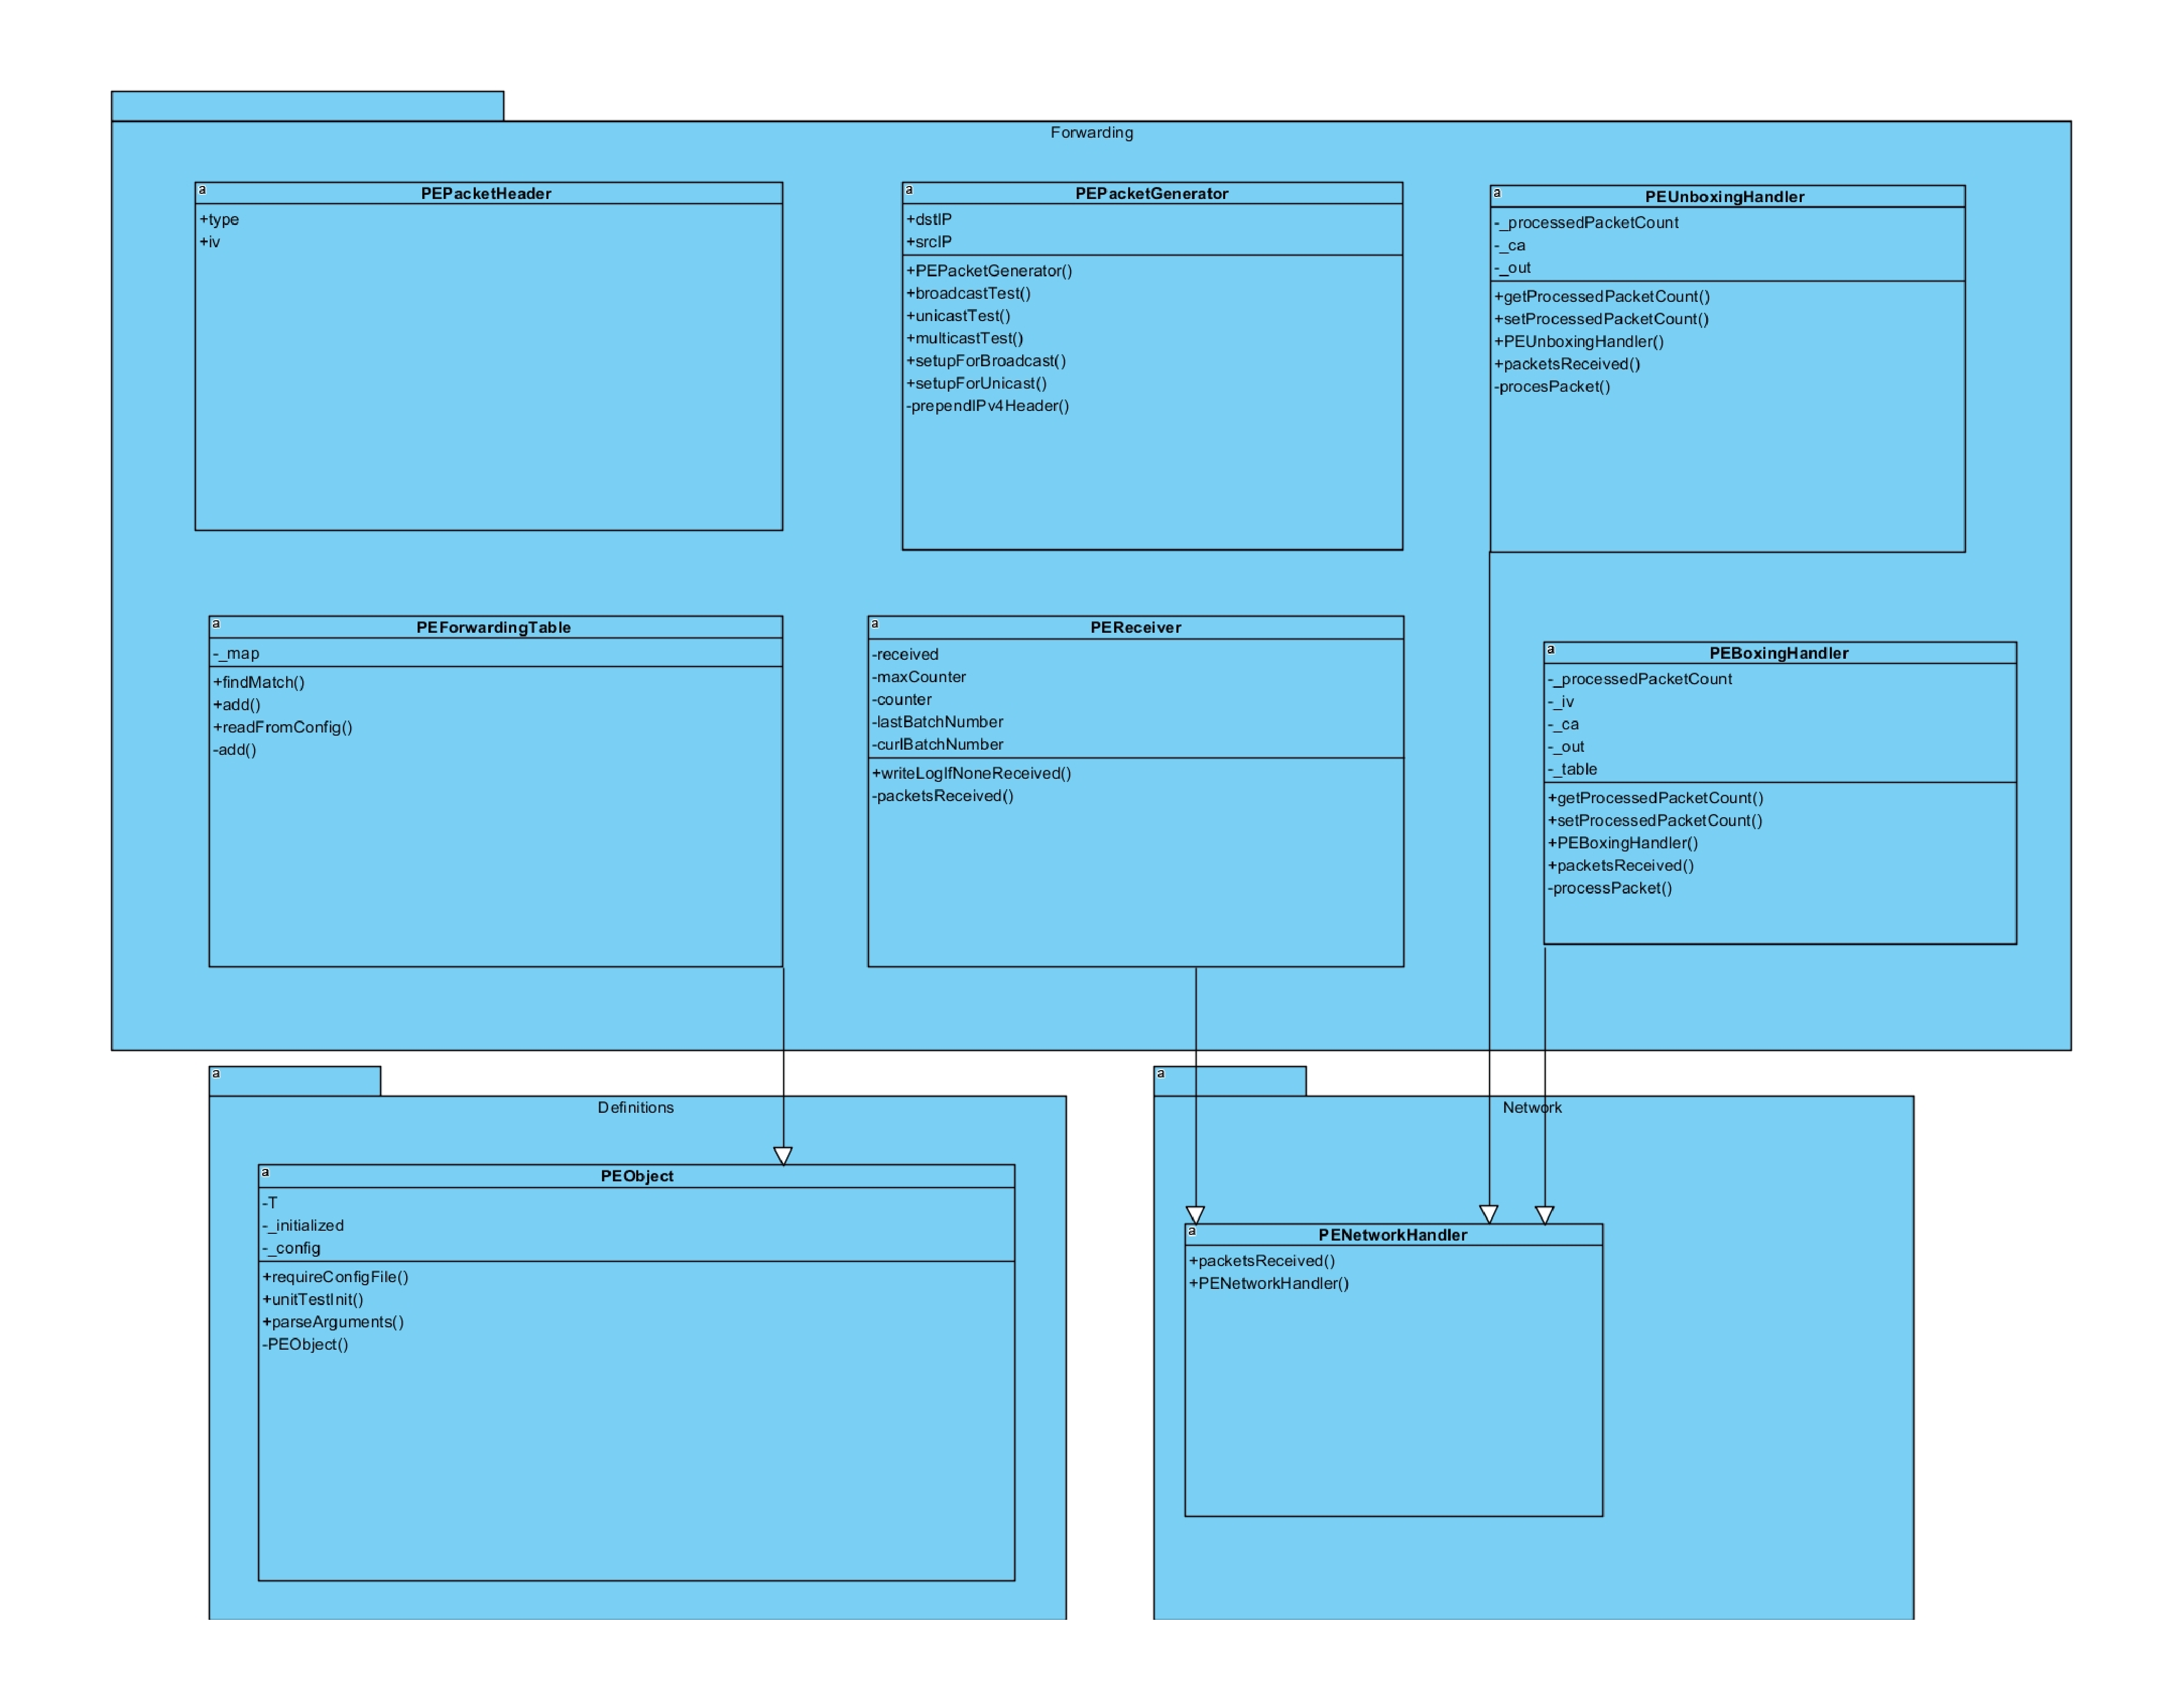
\includegraphics[width=1 \textwidth]{figures/Forwarding.pdf}
		\caption{Forwarding}
	\end{center}
\end{figure}

\begin{description}
	\item[PEForwardingTable]
	Eine \texttt{PEForwardingTable} stellt eine Forwarding Tabelle dar. Sie enthält hierfür Paare von Netzwerkadressen und die dafür zugehörigen MAC-Adressen. Es ist möglich die Einträge aus einer config-Datei einlesen zu lassen.
	
	\item[PEBoxingHandler]
	Ein \texttt{PEBoxingHandler} erbt von \texttt{PENetworkHandler}. Er validiert empfangene Pakete, chiffriert diese und sendet sie nach Abfrage ihres Ziels in \texttt{PEForwardingTable} weiter.
	
	\item[PEUnboxingHandler] 
	Ein \texttt{PEUnboxingHandler} erbt von \texttt{PENetworkHandler}. Er stellt die Gegenseite zum \texttt{PEBoxingHandler} dar, indem er empfangene Pakete validiert und dechiffriert. Danach werden diese ins rote Netz weitergesendet.
	
	\item[PEPacketHeader]
	Der \texttt{PEPacketHeader} ist eine Klasse die dem einfacheren Editieren eines PECTO-Paket Headers dient.
	
	\item[PEPacketGenerator]
	Ein \texttt{PEPacketGenerator} dient zum generieren von Paketen für Testfälle. Es wird hierbei zwischen Broadcast- und Unicast-Paketen unterschieden.
	
	\item[PEReceiver]
	Ein \texttt{PEReceiver} validiert empfangene Pakete und zählt diese zu Testzwecken, um eventuellen Paketverlust zu erkennen.
\end{description}

\subsection{Definitionskomponente}
Die Definitionskomponente stellt diverse Hilfsfunktionen für den Umgang mit Binärdaten bereit.
Zudem wird die Oberklasse für alle PECTO-Komponenten, die ein initialisiertes DPDK voraussetzen, definiert. (siehe Abbildung 4)

\begin{figure}
	\begin{center}
		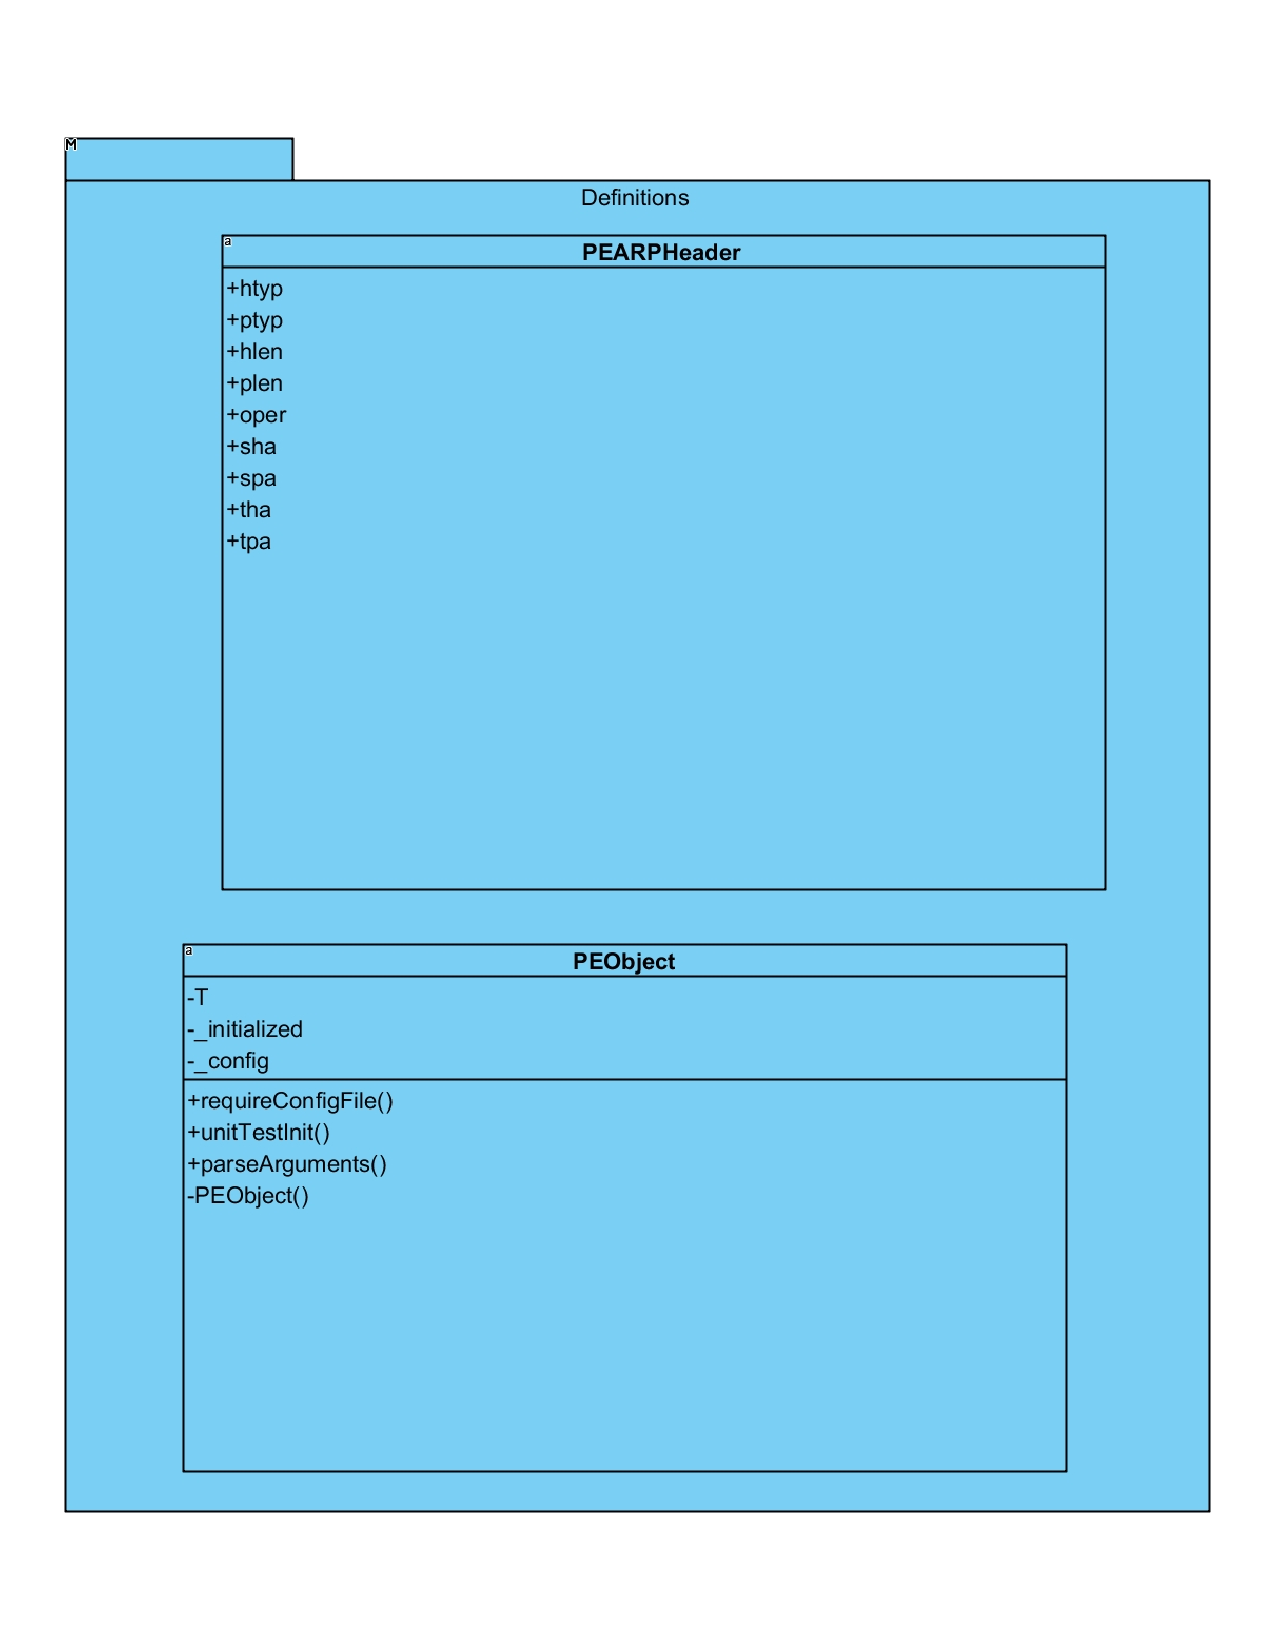
\includegraphics[width=1 \textwidth]{figures/Definitions.pdf}
		\caption{Definitionskomponente}
	\end{center}
\end{figure}

\begin{description}
	\item[PEObject] 
	\texttt{PEObject} stellt die Basisklasse für alle DPDK-abhängigen Komponenten bereit.
	Diese Klasse erbt von \texttt{SOObject} aus der \texttt{coreLib} des Fachgebietes und stellt damit nützliche Funktionen bereit, um Speicherlecks zu finden.
	Sie existiert zur einfacheren Handhabung auch mit einem Template-Parameter, in den stets die abgeleitete Klasse eingesetzt werden muss. 
\end{description}

\subsection{Kryptographiekomponente}
In der Kryptographiekomponente sind die verschiedenen Kryptoalgorithmen gekapselt. (siehe Abbildung 5)

\begin{figure}
	\begin{center}
		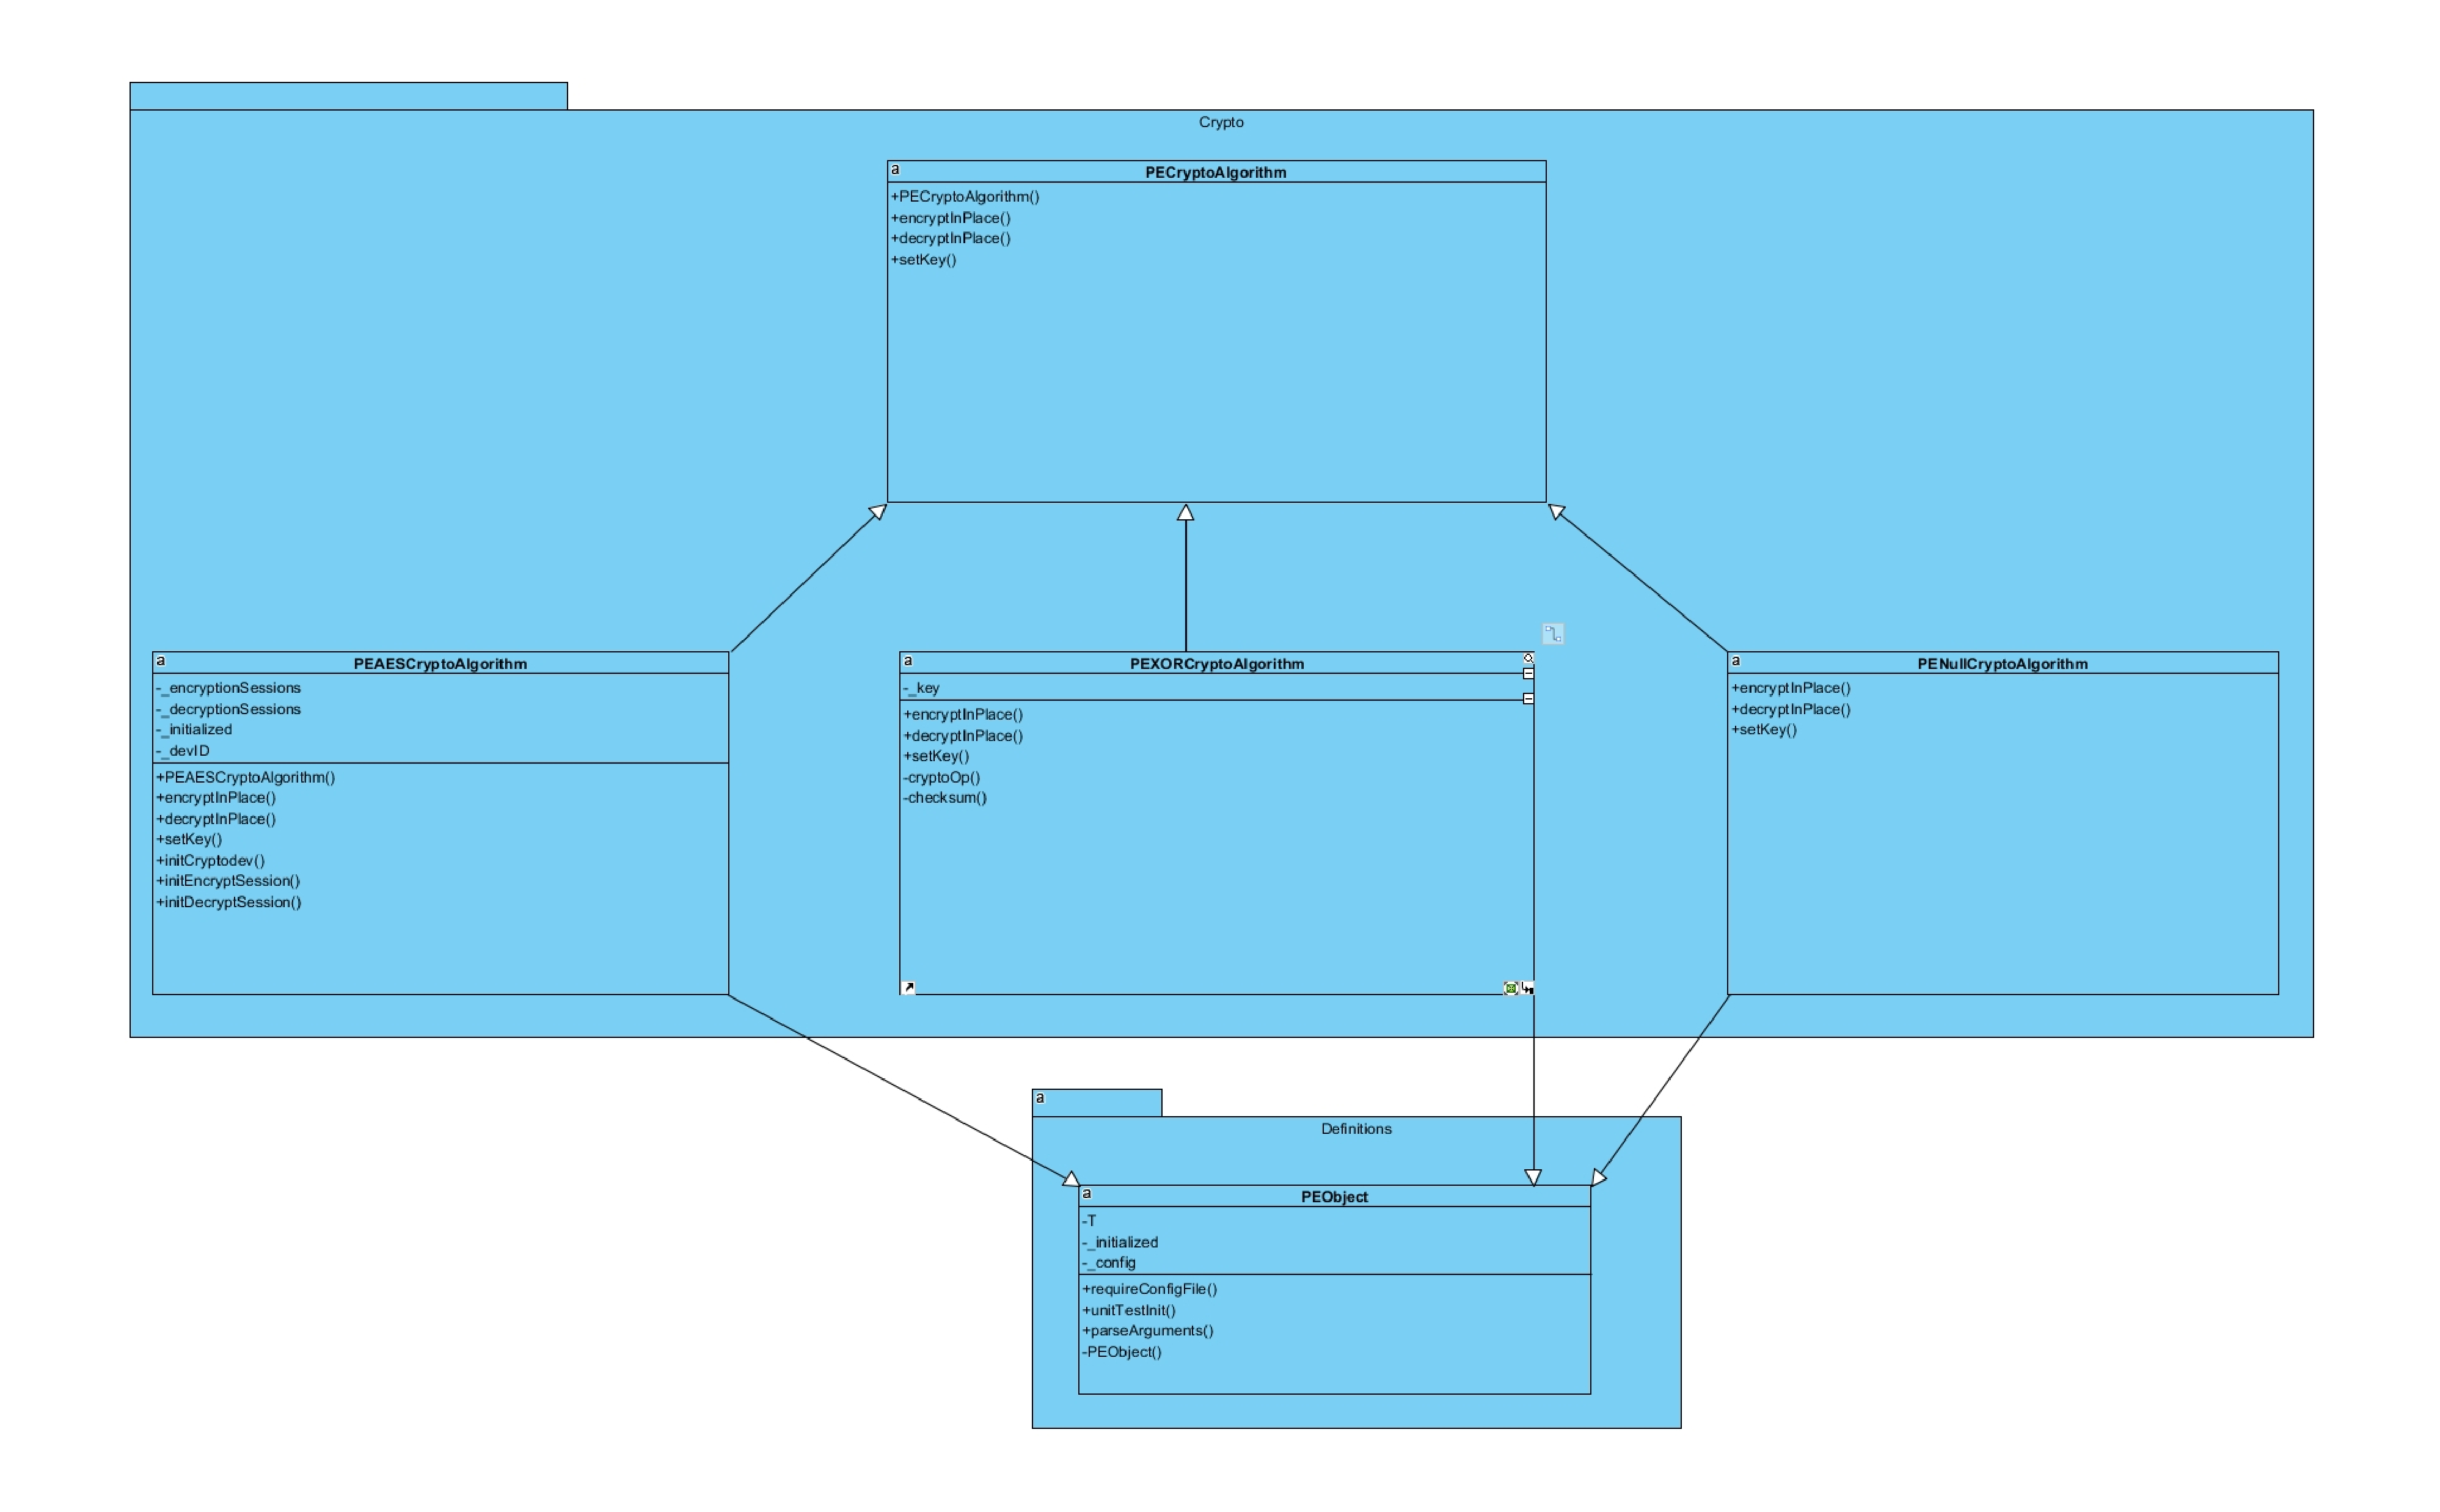
\includegraphics[width=1 \textwidth]{figures/Crypto.pdf}
		\caption{Kryptographiekomponente}
	\end{center}
\end{figure}

\begin{description}
	\item[PECryptoAlgorithm] 
	\texttt{PECryptoAlgorithm} ist das Interface, dass von allen kryptografischen Algorithmen implementiert wird. 
	Es stellt Funktionen zum Setzen eines Schlüssels, sowie zum Ver- und Entschlüsseln bereit.
	
	\item[PENullCryptoAlgorithm]
	Dieser Algorithmus implementiert das Nullchiffre, führt also beim Ver- und Entschlüsseln keinerlei Änderung an den Daten durch.
	
	\item[PEXORCryptoAlgorithm]
	Der XOR-Algorithmus nutzt die XOR-Funktion, um die Daten zu ver- und entschlüsseln.
	Dies ist zwar nicht sicher, kann aber beim Debuggen hilfreich sein.
	
	\item[PEAESCrytoAlgorithm]
	Der AES-Algorithmus kaspelt das vom DPDK bereitgestellte AES-GCM-Verfahren. 
\end{description}

\subsection{Concurrency-Komponente}
Die Concurrency-Komponente stellt Funktionen zur Threaderzeugung und Synchronisation bereit.
Zudem bietet sie Makros, welche die sichere Verwendung von Locks, insbesondere Spinlocks, vereinfachen. (siehe Abbildung 6)

\begin{figure}
	\begin{center}
		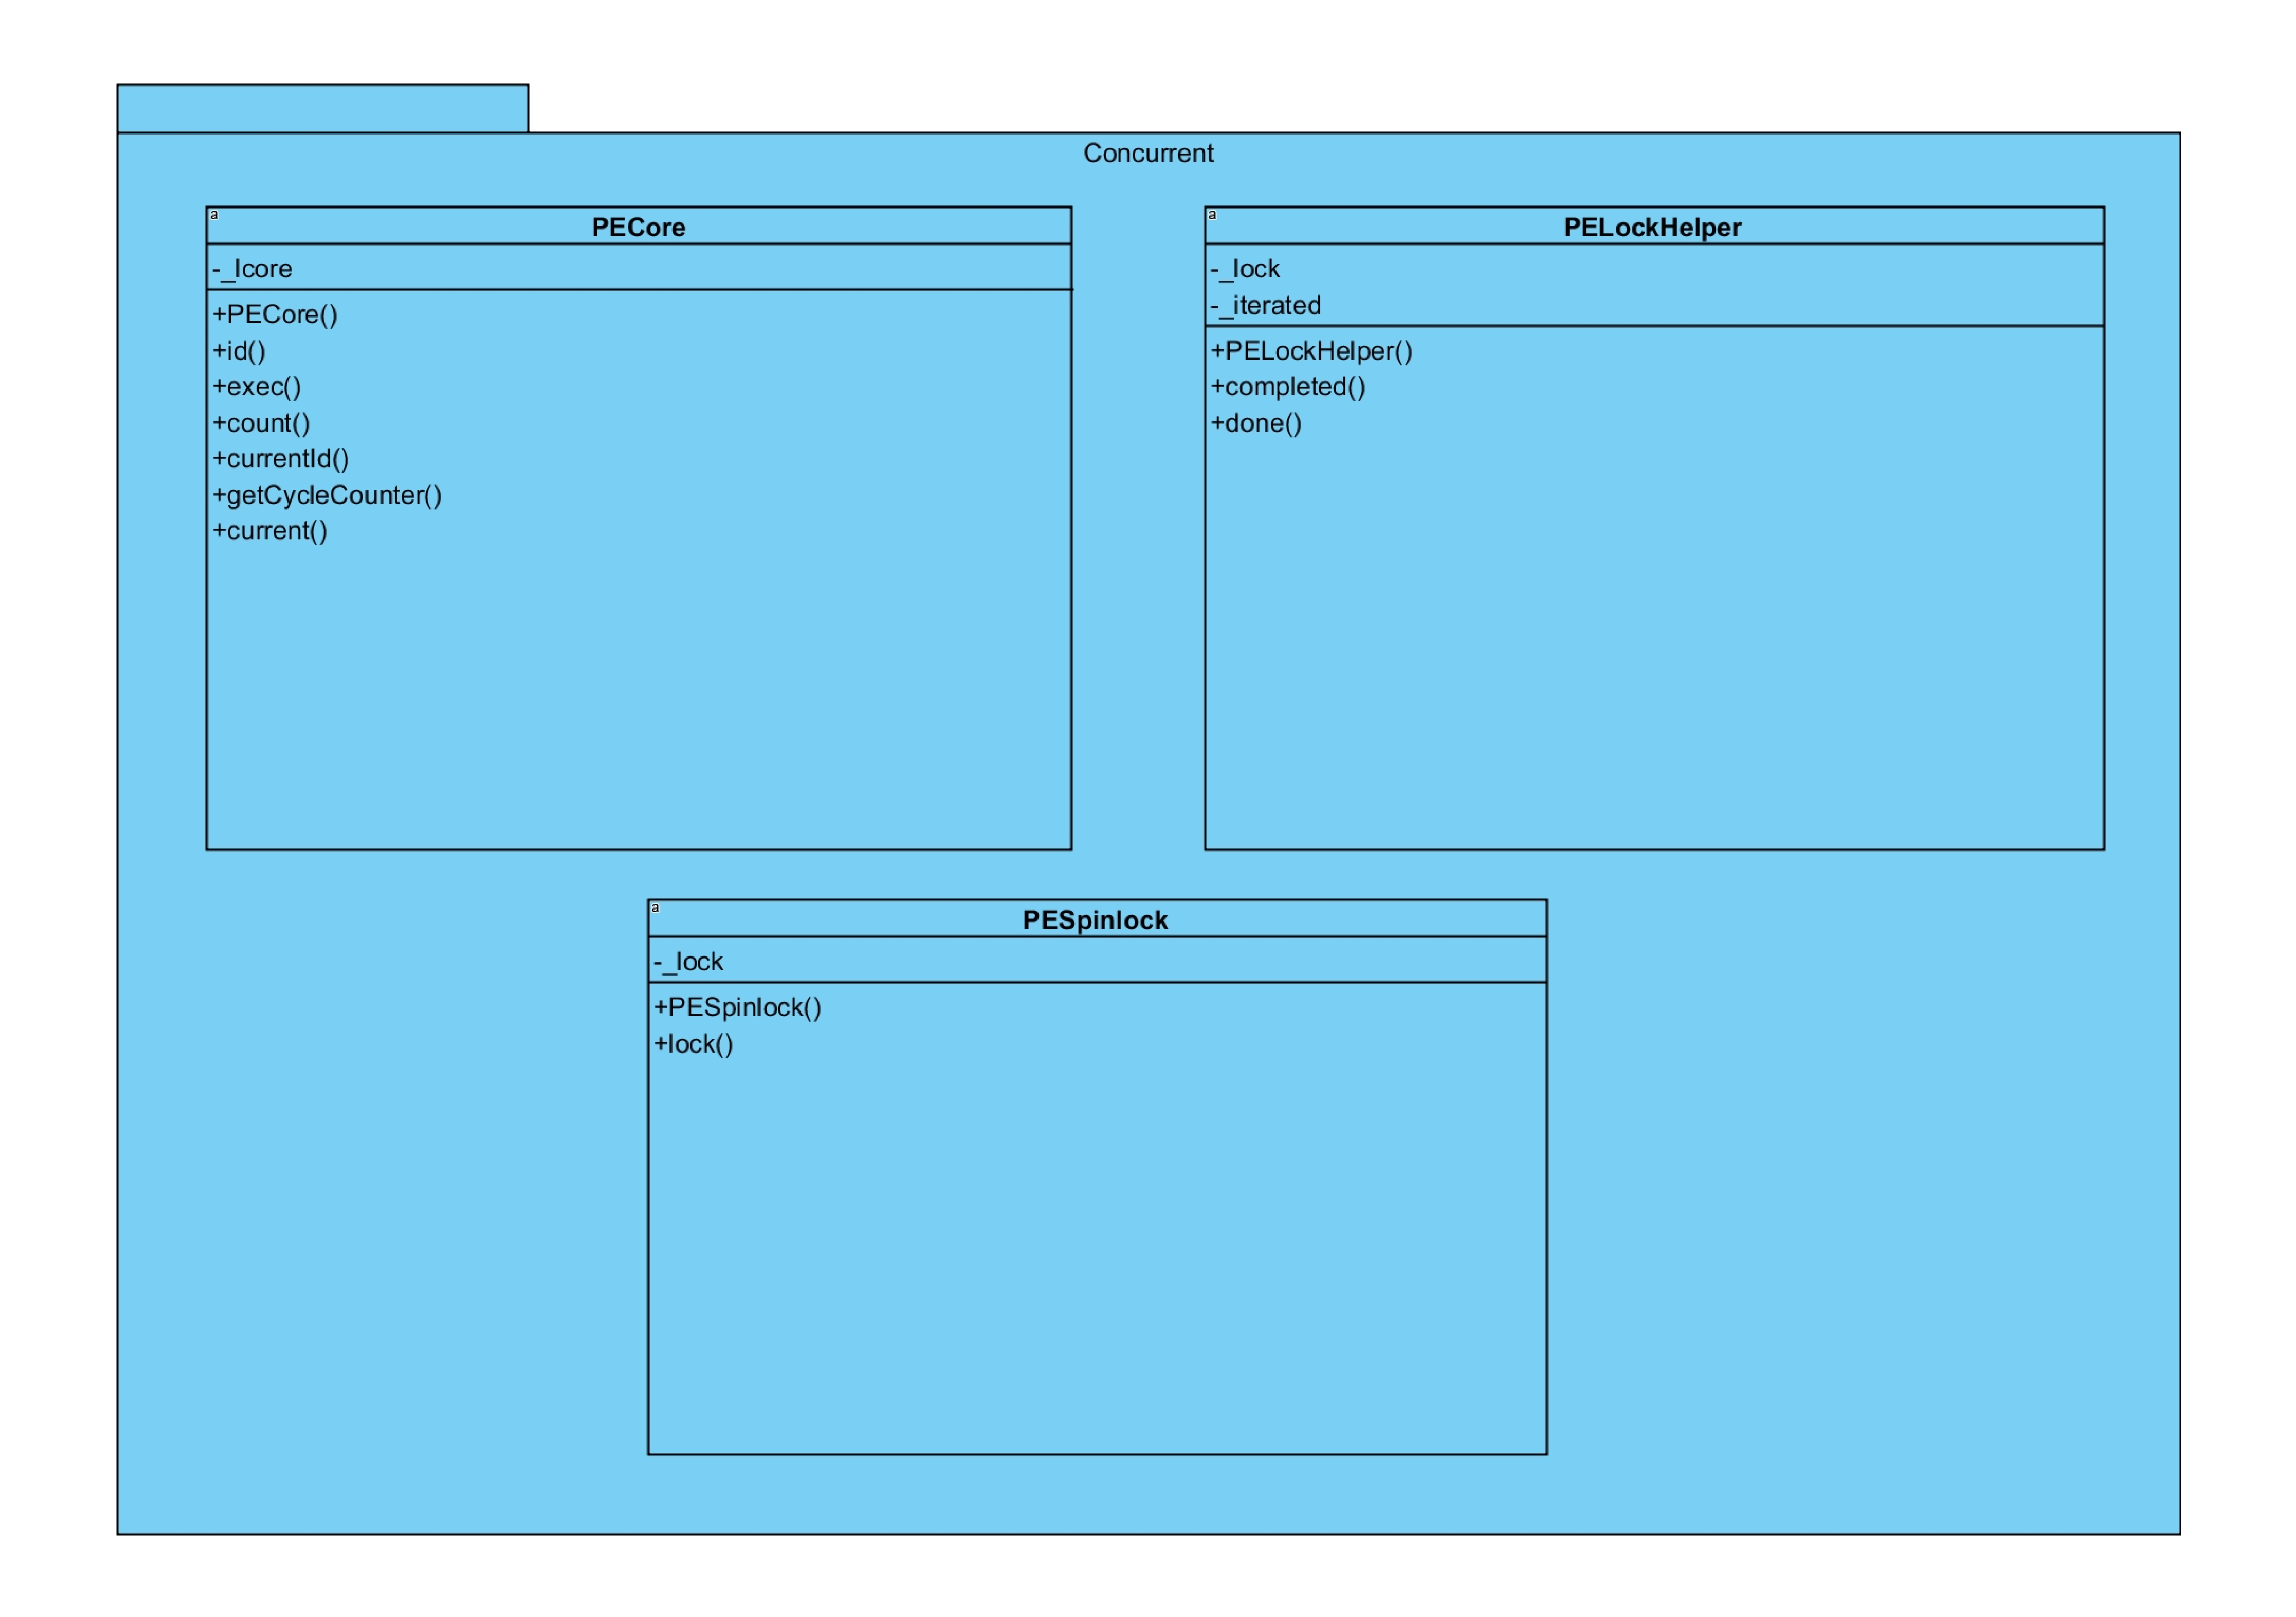
\includegraphics[width=1 \textwidth]{figures/Concurrent.pdf}
		\caption{Concurrency-Komponente}
	\end{center}
\end{figure}

\begin{description}
	\item[PECore] 
	\texttt{PECore} verwaltet die verschieden vom DPDK erzeugten Threads, die jeweils einem Prozessorkern zugewiesen sind.
	
	\item[PESpinlock]
	Der Spinlock implementiert eine einfache Möglichkeit des gegenseitigen Ausschlusses.
	Dabei wird kein rekursives Sperren innerhalb eines Threads zugelassen. 
\end{description}


\clearpage
\section{Ergebnisse der zweiten Iteration} 
Die Ergebnisse aus der zweiten Iteration ergeben sich durch:

\begin{description}
	\leftskip=0,8cm
	\item[Aktualisierter Grobentwurf:] Der Grobentwurf umfasst eine erste Übersicht über die Funktions- und Arbeitsweise des Systems.
	
	\item[Feinentwurf:] Der Feinentwurf beinhaltet einen Überblick über Objekte und Klassenstrukturen, welche das System implementieren.
	Es veranschaulicht außerdem die genaue Funktions- und Arbeitsweise des Systems.
	
	\item[Implementierung:] Die Implementierung wurde fortgeführt und verfeinert.
	Hauptbestandteile, um welche diese erweitert wurde, sind die Realisierung der Verschlüsselung mit statischem Schlüssel und das Forwarding von generierten Paketen zwischen mehreren Instanzen.
	
	\item[Planung:] Es wurden Festlegungen für die letzte Iteration getroffen, hierbei wurde insbesondere das weitere Vorgehen innerhalb des Teams besprochen.
	
\end{description}

\clearpage


\section{Glossar/ Abkürzungen}

\begin{description}
	\item[AES] (Advanced Encryption Standard) ist ein deterministisches Verschlüsselungsverfahren, bei dem durch einen Schlüssel ein Text fester Länge in ein Chiffre fester Länge transformiert wird. 
	
	\item[AES-NI] (Advanced Encryption Standard New Instructions) ist eine Erweiterung zur x86-Befehlssatzarchitektur für Mikroprozessoren von Intel und AMD. Man kann hiermit eine Verbesserung der Geschwindigkeit von Anwendungen, welche AES-Ver- und Entschlüsselungen nutzen, erzielen. 
	
	\item[ARP] (Address Resolution Protocol) ist ein Protokoll, mit dem Netzwerkadressen auf Hardwareadressen abgebildet werden können, damit eine Kommunikation auf dem Network Layer stattfinden kann.  
	
	\item[Chiffre] ist ein Geheimtext, der unter Verwendung eines Schlüssels mit kryptographischen Verfahren derart verändert wurde, dass es nicht mehr möglich ist, dessen Inhalt zu verstehen.
	
	\item[CPH] (Control Paket Hub) regelt die Verarbeitung von Schlüsselpaketen innerhalb PECTOs.
	
	\item[cxxtests] ist ein Framework, welches zur Erstellung von Unit-Tests verwendet wird.
	
	\item[Dispatch-Komponente] steuert die Einteilung der Pakete (verschlüsselt/unverschlüsselt) für das System.
	
	\item[DPDK] (Data Plane Development Kit) ist eine Sammlung von Bibliotheken und Netzwerkkontrolltreibern, die zur schnellen Paketverarbeitung genutzt werden kann.
	
	\item[EAL] (Environment Abstraction Layer) ist eine Hardwareabstraktionsschicht, die erzeugt wird, um direkte Anfragen an die Hardware leichter zu stellen und die allgemeine Nutzung zu vereinfachen.
		
	\item[Effizienz] ist das Ausmaß der Sparsamkeit des Systems bezüglich seiner Ressourcen. Ziel sind insbesondere ein geringer Speicherverbrauch, eine geringe CPU-Last und eine hohe Paketrate.
	
	\item[IV-Space] ist der separiete Zahlenraum, welcher jeder Instanz des Systems individuell zugeordnet wird, um unterschiedliche Initialisierungsvektoren zu erstellen.
	
	\item[Layer-2-Switch] ist ein einfaches Kopplungsgerät, das lokale Netzwerksegmente miteinander verbindet und eine Weiterleitfunktion der Datenpakete, auf dem Data Link Layer, übernimmt. 
	Sie haben insbesondere keine Vermittlungs- und Routingfunktionen.  
	
	\item[Logging] ist das automatische Speichern von Datenänderungen, welche in Logdateien hinterlegt werden.
	
	\item[Mock] ist ein Objekt, welches das Verhalten eines realen Objektes nachbildet, und für Unit-Tests verwendet wird.
	
	\item[Network Abstraction-Komponente] abstrahiert die Verwendung des DPDK und bildet die Schnittstelle zum übrigen System.
	
	\item[Paketdurchsatz] ist die Anzahl der Pakete, die in einer bestimmten Zeit gesendet werden können.
	
	\item[Passphrase] ist eine Zeichenfolge, über die der Zugriff auf ein Netzwerk gesteuert wird.
	
	\item[Portabilität] ist die Möglichkeit das System auf einem anderen Betriebssystem einzusetzen.
	
	\item[Robustheit] ist die Fähigkeit, auch unter ungünstigen Bedingungen zuverlässig zu funktionieren. Sie dürfen zu keinerlei Problemen führen.
	
	\item[Sicherheit] ist die Fähigkeit, dass Systemfunktionen nicht von einer dritten Person abgehört oder manipuliert werden können.
	
	\item[Skalierbarkeit] ist die Fähigkeit eines Systems, die Leistung durch das Hinzufügen von Ressourcen zu steigern.
	
	\item[Unit-Test] ist ein Test, der verwendet wird, um Einzelteile von Computerprogrammen auf korrekte Funktionalität zu testen.
	
	\item[Zuverlässigkeit] ist die Fähigkeit, dass ein Programm während einer gewissen Betriebsdauer nur begrenzt viele Fehlerfälle aufweisen darf.
	
	\item[Polling] bezeichnet in der Informatik die Methode, den Status eines Geräts aus Hard- oder Software oder das Ereignis einer Wertänderung mittels zyklischem Abfragen zu ermitteln.
	
	\item[GCM] ist ein Betriebsmodus, in der Blockchiffren für eine symmetrische Verschlüsselungsanwendung betrieben werden können
	
	\item[Bug] bezeichnet im Allgemeinen ein Fehlverhalten von Computerprogrammen.
	
	\item[VPN] steht für Virtual Private Network. Dient dazu, Teilnehmer des bestehenden Kommunikationsnetzes an ein anderes Netz zu binden.
	
	\item[Memory Pool] ist ein dynamischer Speicher mit festen Blockgrößen.                                     
	
	  
\end{description}


%\section{Referenzen}

  
\end{document}
